\clearpage
\renewcommand{\sectionprefix}{C.2}  % Set prefix for this question
\setcounter{subsection}{0}  % Reset subsection counter
\section*{Section C: Question 2}
\markboth{Section C: Question 2}{Section C: Question 2}
\addcontentsline{toc}{section}{Section C: Question 2}
\renewcommand{\subsectionmark}[1]{}

\textbf{Problem Statement:} The case below (figure on the left) represents a typical short-circuit fault in transmission lines and the breaker operation for line interruption. The equivalent circuit is shown in the figure on the right.

\begin{figure}[h!]
    \centering
    \begin{minipage}{0.45\textwidth}
        \centering
        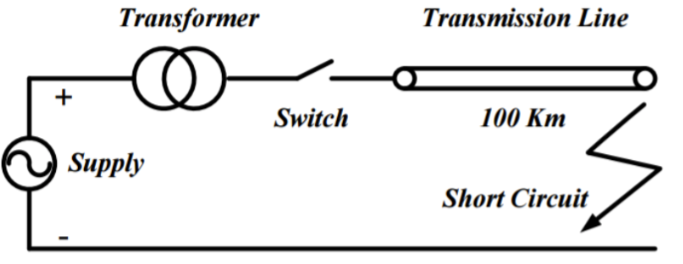
\includegraphics[width=\textwidth]{figures/figure-C-circuit-left.png}
        \caption{Transmission line with short-circuit fault}
        \label{fig:c02_circuit_left}
    \end{minipage}
    \hfill
    \begin{minipage}{0.45\textwidth}
        \centering
        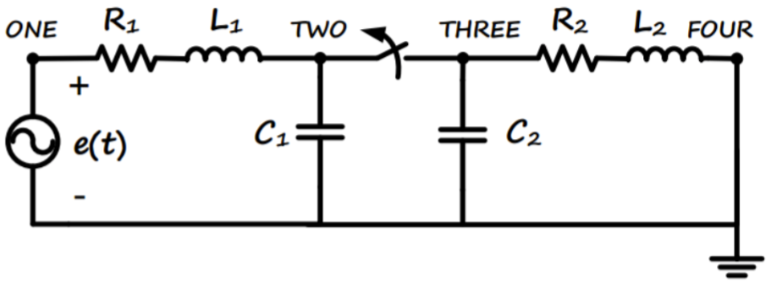
\includegraphics[width=\textwidth]{figures/figure-C-circuit-right.png}
        \caption{Equivalent circuit representation}
        \label{fig:c02_circuit_right}
    \end{minipage}
\end{figure}

On the left-hand side of the switch/breaker, we have the source voltage and a resistance and inductance representing the supply system combined with the transformer. The capacitor to the left of the breaker represents the combined substation capacitance due to the substation busbars. On the right-hand side of the breaker, we have the transmission line parameters: resistance, inductance, and capacitance represented as simple lumped parameters, where the right side is short-circuited due to the fault, assuming that the fault has already been applied. We have assumed a single-phase circuit here for simplicity. The parameters of the circuit below are: $e(t) = 230\times\cos(\omega t)$ kV, $\omega=377$ rad/s, $R_1=3\Omega$, $L_1=350$ mH, $R_2=50\Omega$, $L_2=100$ mH, $C_1=10$ nF, $C_2=600$ nF. Assume that the system is operating with zero initial conditions and the breaker is initially closed. At $t=8$ ms, the breaker is commanded to open the line, but it will not actually open until the current passes through zero. The study period is from $t=0$ to $t=20$ ms.

2) Write your own MATLAB code to solve the system and also obtain the solution using PSCAD.

\noindent\rule{\textwidth}{0.4pt}

\vspace{1em}

\textbf{Solution:}

\subsection{Nodal Analysis and Equivalent Circuit Diagrams}

To implement the MATLAB solution, we first need to establish the equivalent circuit diagrams for the nodal analysis method. The circuit behavior changes based on the breaker state.

\begin{figure}[H]
    \centering
    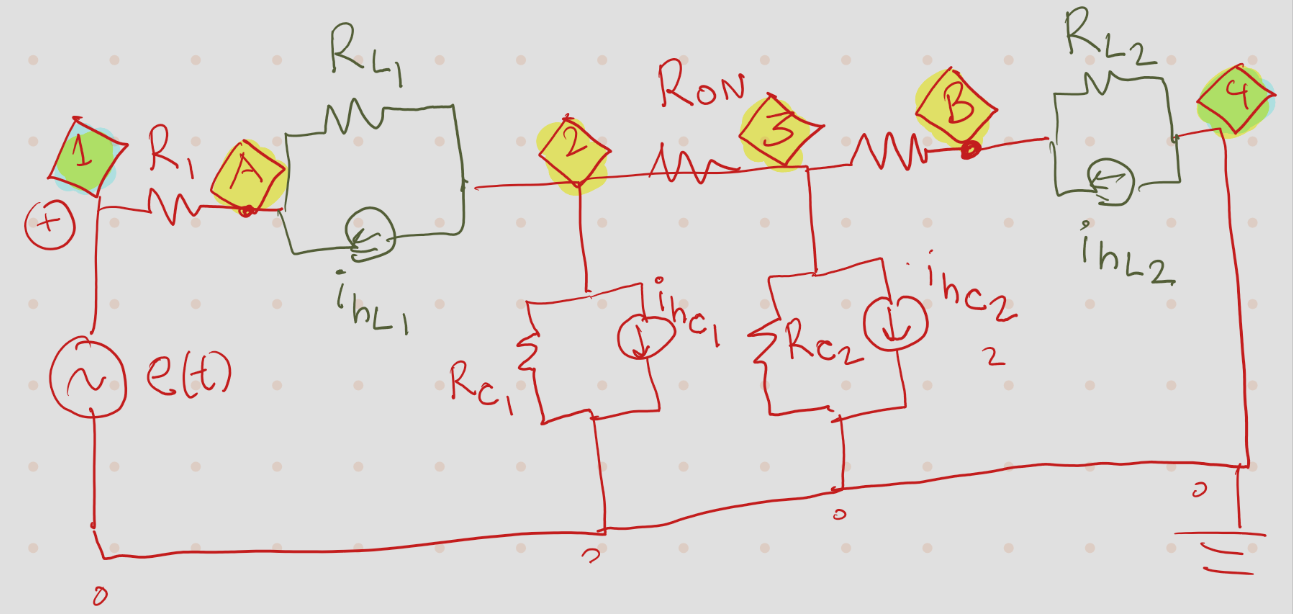
\includegraphics[width=0.85\textwidth]{figures/qC-nodal-ckt-equiv-diag-swt-closed-handdrawn.png}
    \caption{Equivalent circuit diagram for nodal analysis when switch is closed (breaker closed state). Note that the nodes highlighted in green are connected to voltage sources or ground, while those in yellow are unknowns. This configuration will be used to construct the conductance matrix $\mathbf{G}$ for $t < t_{\text{open, actual}}$.}
    \label{fig:c02_nodal_closed}
\end{figure}

\begin{figure}[H]
    \centering
    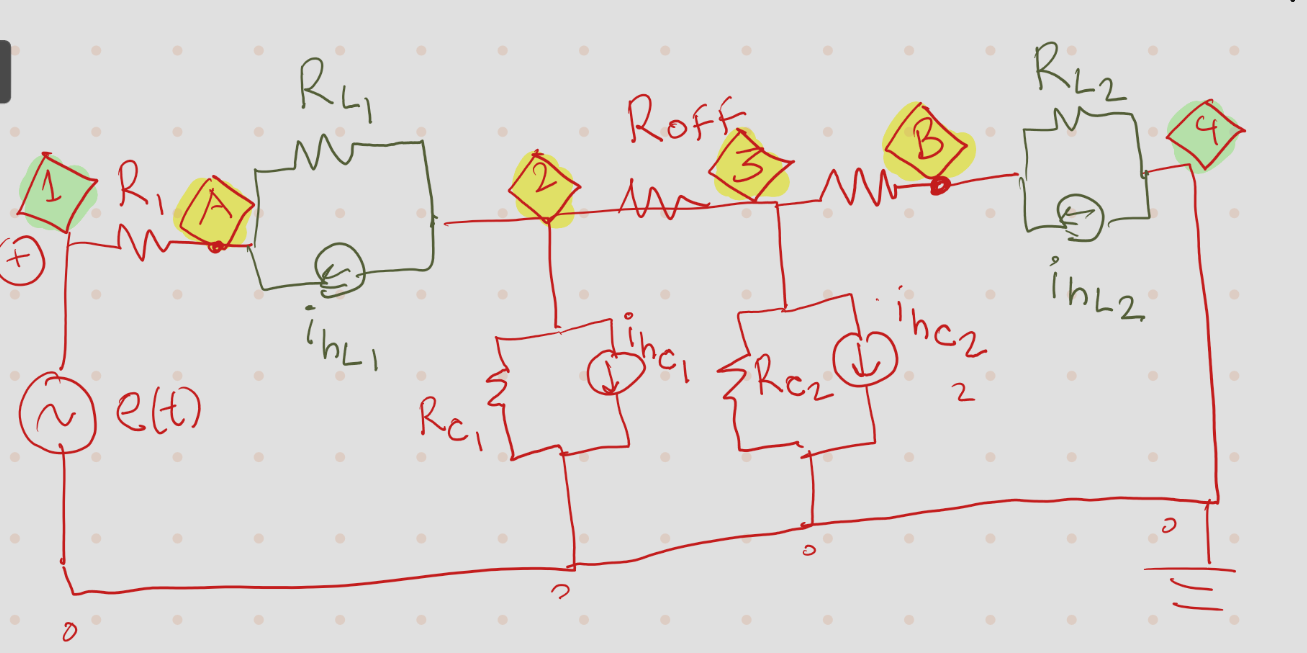
\includegraphics[width=0.85\textwidth]{figures/qC-nodal-ckt-equiv-diag-swt-opened-handdrawn.png}
    \caption{Equivalent circuit diagram for nodal analysis when switch is opened (breaker open state). Note that the nodes highlighted in green are connected to voltage sources or ground, while those in yellow are unknowns.This configuration will be used to construct the conductance matrix $\mathbf{G}$ for $t \geq t_{\text{open, actual}}$.}
    \label{fig:c02_nodal_open}
\end{figure}

These equivalent circuit diagrams show the companion models for the inductors and capacitors, which will be referenced when building the conductance matrices $\mathbf{G}$ for the nodal analysis formulation.

% Your solution here

\vspace{1em}
\noindent\rule{\textwidth}{0.4pt}